% ============================================================
%  AlphaStream India -- Architecture & Impact Model
%  ET AI Hackathon 2026 -- Problem Statement 6
%  Secondary Submission Document
% ============================================================
\documentclass[11pt, a4paper]{article}

% -- Core packages -----------------------------
\usepackage[a4paper, top=2.2cm, bottom=2.2cm,
            left=2.4cm, right=2.4cm, headheight=14pt]{geometry}
\usepackage[T1]{fontenc}
\usepackage[utf8]{inputenc}
\DeclareUnicodeCharacter{20B9}{\Rs}
\newcommand{\Rs}{Rs.\,}
% -- Fonts: Source family (modern, clean, professional) ------
\usepackage[default]{sourceserifpro}
\usepackage[scale=0.95]{sourcesanspro}
\usepackage[scale=0.92]{sourcecodepro}
\usepackage{microtype}
\usepackage{parskip}
\usepackage{setspace}
\usepackage{graphicx}

% -- Color ----------------------------------
\usepackage{xcolor}
\definecolor{navy}{RGB}{26,  58, 107}
\definecolor{cyan}{RGB}{ 0, 180, 216}
\definecolor{teal}{RGB}{ 0, 128, 128}
\definecolor{green}{RGB}{45, 156,  77}
\definecolor{orange}{RGB}{230, 126, 34}
\definecolor{purple}{RGB}{142,  68, 173}
\definecolor{red}{RGB}{192,  57,  43}
\definecolor{steel}{RGB}{ 52,  73,  94}
\definecolor{lgray}{RGB}{248, 248, 248}
\definecolor{mgray}{RGB}{170, 170, 170}
\definecolor{gold}{RGB}{241, 196, 15}
\definecolor{darkgreen}{RGB}{39, 174, 96}

% -- TikZ -----------------------------------
\usepackage{tikz}
\usetikzlibrary{
  shapes.geometric, shapes.multipart,
  arrows.meta, positioning, fit,
  backgrounds, calc, shadows.blur
}

% -- Tables ----------------------------------
\usepackage{booktabs}
\usepackage{tabularx}
\usepackage{array}
\usepackage{multirow}
\usepackage{colortbl}

% -- Layout / headings --------------------------
\usepackage{titlesec}
\usepackage{fancyhdr}
\usepackage{float}
\usepackage{caption}
\usepackage{enumitem}
\usepackage{amsmath}

% -- Boxes ----------------------------------
\usepackage{tcolorbox}
\tcbuselibrary{skins, breakable}

% -- Links ----------------------------------
\usepackage[hidelinks, colorlinks=true, linkcolor=navy, urlcolor=cyan!70!black]{hyperref}

% ============================================================
%  Section formatting
% ============================================================
\setstretch{1.15}

\titleformat{\section}
  {\Large\bfseries\sffamily\color{navy}}
  {\thesection.}{0.6em}{}
  [\vspace{0pt}\color{cyan}\rule{\linewidth}{1.5pt}\vspace{2pt}]

\titleformat{\subsection}
  {\large\bfseries\sffamily\color{navy!85}}
  {\thesubsection}{0.5em}{}

\titleformat{\subsubsection}
  {\normalsize\bfseries\sffamily\color{navy!70}}
  {\thesubsubsection}{0.5em}{}

\titlespacing{\section}{0pt}{1.2em}{0.5em}
\titlespacing{\subsection}{0pt}{0.9em}{0.35em}
\titlespacing{\subsubsection}{0pt}{0.7em}{0.25em}

% ============================================================
%  Header / footer
% ============================================================
\pagestyle{fancy}
\fancyhf{}
\fancyhead[L]{\small\color{navy}\textbf{AlphaStream India -- Architecture \& Impact}}
\fancyhead[R]{\small\color{mgray}ET AI Hackathon 2026}
\fancyfoot[C]{\small\color{navy}\thepage}
\renewcommand{\headrulewidth}{0.5pt}
\renewcommand{\headrule}{\color{cyan}\hrule width\headwidth height 0.5pt}

% ============================================================
%  tcolorbox styles
% ============================================================
\newtcolorbox{infobox}[1][]{
  enhanced, colback=cyan!6, colframe=cyan!50!navy,
  boxrule=0.7pt, arc=4pt,
  left=7pt, right=7pt, top=5pt, bottom=5pt,
  fonttitle=\bfseries\sffamily\color{white},
  attach boxed title to top left={yshift=-2mm, xshift=4mm},
  boxed title style={colback=cyan!50!navy, arc=3pt, boxrule=0pt},
  #1}

\newtcolorbox{greenbox}[1][]{
  enhanced, colback=green!6, colframe=green!60!black,
  boxrule=0.7pt, arc=4pt,
  left=7pt, right=7pt, top=5pt, bottom=5pt,
  fonttitle=\bfseries\sffamily\color{white},
  attach boxed title to top left={yshift=-2mm, xshift=4mm},
  boxed title style={colback=green!60!black, arc=3pt, boxrule=0pt},
  #1}

\newtcolorbox{orangebox}[1][]{
  enhanced, colback=orange!6, colframe=orange!60!black,
  boxrule=0.7pt, arc=4pt,
  left=7pt, right=7pt, top=5pt, bottom=5pt,
  fonttitle=\bfseries\sffamily\color{white},
  attach boxed title to top left={yshift=-2mm, xshift=4mm},
  boxed title style={colback=orange!60!black, arc=3pt, boxrule=0pt},
  #1}

\newtcolorbox{keymetricbox}{
  enhanced, colback=navy!5, colframe=navy!70,
  boxrule=1pt, arc=6pt,
  left=10pt, right=10pt, top=8pt, bottom=8pt}

% ============================================================
%  TikZ styles
% ============================================================
\tikzset{
  layerA/.style={draw=steel!70!black, fill=steel!12,
    rounded corners=5pt, minimum width=12.4cm, minimum height=1.4cm,
    text width=12.0cm, align=center, font=\small},
  layerB/.style={draw=navy!70!black, fill=navy!10,
    rounded corners=5pt, minimum width=12.4cm, minimum height=1.4cm,
    text width=12.0cm, align=center, font=\small},
  layerC/.style={draw=purple!60!black, fill=purple!8,
    rounded corners=5pt, minimum width=12.4cm, minimum height=1.4cm,
    text width=12.0cm, align=center, font=\small},
  layerD/.style={draw=green!60!black, fill=green!8,
    rounded corners=5pt, minimum width=12.4cm, minimum height=1.4cm,
    text width=12.0cm, align=center, font=\small},
  layerE/.style={draw=red!60!black, fill=red!8,
    rounded corners=5pt, minimum width=12.4cm, minimum height=1.4cm,
    text width=12.0cm, align=center, font=\small},
  mainarrow/.style={->, >=Stealth, line width=1.4pt, color=navy!65},
  subarrow/.style={->, >=Stealth, line width=0.9pt, color=navy!45},
  sidarrow/.style={->, >=Stealth, line width=0.9pt, color=cyan!70!navy, dashed}
}

% ============================================================
%  Helpers
% ============================================================
\newcolumntype{L}[1]{>{\raggedright\arraybackslash}p{#1}}
\newcolumntype{C}[1]{>{\centering\arraybackslash}p{#1}}

% ============================================================
\begin{document}

% -- Title page -------------------------------
\begin{titlepage}
  \centering
  \vspace*{2cm}

  {\color{cyan}\rule{\linewidth}{2.5pt}}
  \vspace{0.8cm}

  {\fontsize{28}{34}\selectfont\bfseries\color{navy}
    AlphaStream India}\\[0.5cm]
  {\LARGE\color{steel}
    Architecture Document \& Impact Model}

  \vspace{0.5cm}
  {\color{cyan}\rule{\linewidth}{2.5pt}}

  \vspace{1.5cm}

  % Key stats
  
\begin{tikzpicture}
    \node[fill=navy!8, rounded corners=8pt, inner sep=14pt, text width=13cm, align=center] {
      \begin{tabular}{ccccc}
        {\Large\bfseries\color{navy}13} & {\Large\bfseries\color{navy}$<$2s} &
        {\Large\bfseries\color{navy}30+} & {\Large\bfseries\color{navy}5} &
        {\Large\bfseries\color{navy}14Cr+} \\[2pt]
        {\scriptsize\color{steel}AI Agents} & {\scriptsize\color{steel}News-to-Signal} &
        {\scriptsize\color{steel}API Endpoints} & {\scriptsize\color{steel}Tab Terminal} &
        {\scriptsize\color{steel}Target Users}
      \end{tabular}
    };
  \end{tikzpicture}

  \vspace{1.5cm}

  \begin{infobox}[title={Document Purpose}]
  This document provides:
  \begin{enumerate}[leftmargin=1.4em, itemsep=2pt]
    \item A \textbf{1--2 page architecture diagram and description} showing agent roles,
          how they communicate, tool integrations, and error-handling logic.
    \item A \textbf{quantified impact model} estimating business impact: time saved,
          cost reduced, revenue recovered -- with stated assumptions.
  \end{enumerate}
  \end{infobox}

  \vspace{1.2cm}

  \begin{tabular}{ll}
    \textbf{\color{navy}Competition:}  & ET AI Hackathon 2026 -- Avataar.ai + Unstop \\[3pt]
    \textbf{\color{navy}Problem:}      & PS-6: AI for the Indian Investor \\[3pt]
    \textbf{\color{navy}Repository:}   & \url{https://github.com/wildcraft958/AlphaStream_India} \\[3pt]
    \textbf{\color{navy}Date:}         & March 2026 \\
  \end{tabular}

  \vfill
  {\color{cyan}\rule{\linewidth}{1.5pt}}
\end{titlepage}

% ============================================================
%  PART 1: ARCHITECTURE DOCUMENT
% ============================================================

\section{System Architecture Overview}

AlphaStream India implements a \textbf{streaming RAG + multi-agent} architecture focused
on the Indian equity market (NSE/BSE). The system ingests data from 10+ sources in
real-time, processes it through 13 specialized AI agents, stores structured analytics
in DuckDB, and delivers actionable signals via a Bloomberg-style React terminal.

\subsection{Five-Layer Architecture Diagram}

\begin{figure}[H]
\centering
\begin{tikzpicture}[node distance=0.4cm]

  \node[layerA] (datasrc)
    {\textbf{\color{steel!80!black}Layer 1 -- Indian \& Global Data Sources}\\[2pt]
     \small NSE OHLCV \quad BSE Filings \quad FII/DII (NSDL) \quad Groww \quad
     WorldMonitor \quad FRED \quad NewsAPI \quad RSS};

  \node[layerB, below=0.4cm of datasrc] (pathway)
    {\textbf{\color{navy}Layer 2 -- Pathway Streaming Engine}\\[2pt]
     \small ConnectorSubject \quad Adaptive RAG (xpacks.llm) \quad DocumentStore \quad
     pw.io.subscribe \quad UsearchKnn};

  \node[layerC, below=0.4cm of pathway] (agents)
    {\textbf{\color{purple!80!black}Layer 3 -- Multi-Agent Reasoning (13 Agents)}\\[2pt]
     \small Sentiment \textbullet{} Technical \textbullet{} Risk \textbullet{} Pattern \textbullet{}
     Backtest \textbullet{} Flow \textbullet{} Filing \textbullet{}
     Insider \textbullet{} Anomaly \textbullet{} Search \textbullet{} Chart \textbullet{}
     Report \textbullet{} Decision};

  \node[layerD, below=0.4cm of agents] (analytics)
    {\textbf{\color{green!60!black}Layer 4 -- DuckDB Analytics + NLQ Engine}\\[2pt]
     \small fact/dim tables \quad Pre-aggregated views \quad
     LangGraph Text2SQL \quad ChromaDB \quad MCP Servers};

  \node[layerE, below=0.4cm of analytics] (frontend)
    {\textbf{\color{red!70!black}Layer 5 -- FastAPI + React Terminal (5 Tabs)}\\[2pt]
     \small REST (30+ endpoints) \quad WebSocket \quad SSE \quad
     Overview \textbullet{} Signals \textbullet{} Global \textbullet{} Company \textbullet{} Portfolio};

  \draw[mainarrow] (datasrc.south) -- (pathway.north);
  \draw[mainarrow] (pathway.south) -- (agents.north);
  \draw[mainarrow] (agents.south) -- (analytics.north);
  \draw[mainarrow] (analytics.south) -- (frontend.north);

  \node[right=0.3cm of datasrc,  font=\tiny\color{mgray}, align=left] {Real-time\\ingestion};
  \node[right=0.3cm of pathway,  font=\tiny\color{mgray}, align=left] {Streaming\\callbacks};
  \node[right=0.3cm of agents,   font=\tiny\color{mgray}, align=left] {Signal\\fusion};
  \node[right=0.3cm of analytics, font=\tiny\color{mgray}, align=left] {SQL\\queries};

\end{tikzpicture}
\caption{AlphaStream India -- Five-Layer System Architecture}
\end{figure}

\subsection{Architecture Diagrams}

\begin{figure}[H]
  \centering
  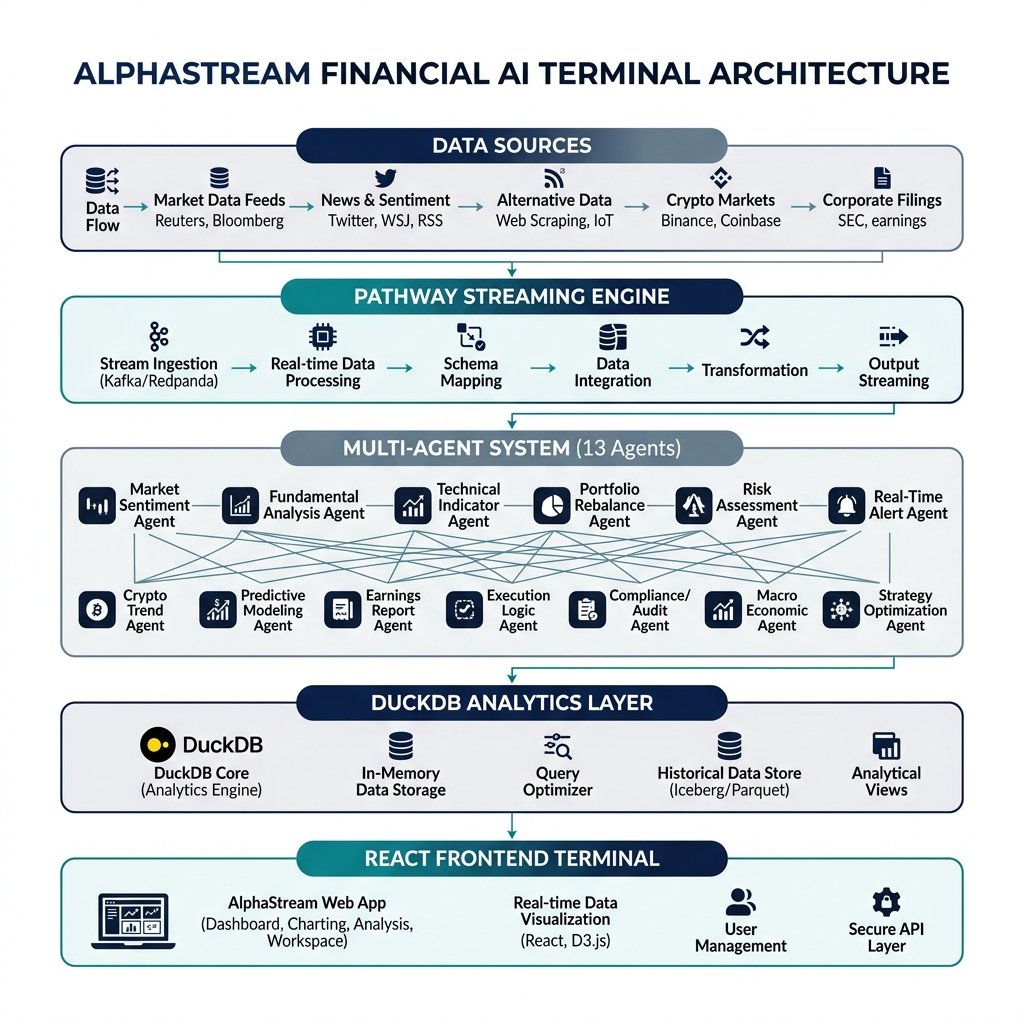
\includegraphics[width=0.92\textwidth]{system_architecture.png}
  \caption{Detailed System Architecture -- Data flow from Indian sources through all processing layers}
\end{figure}

\begin{figure}[H]
  \centering
  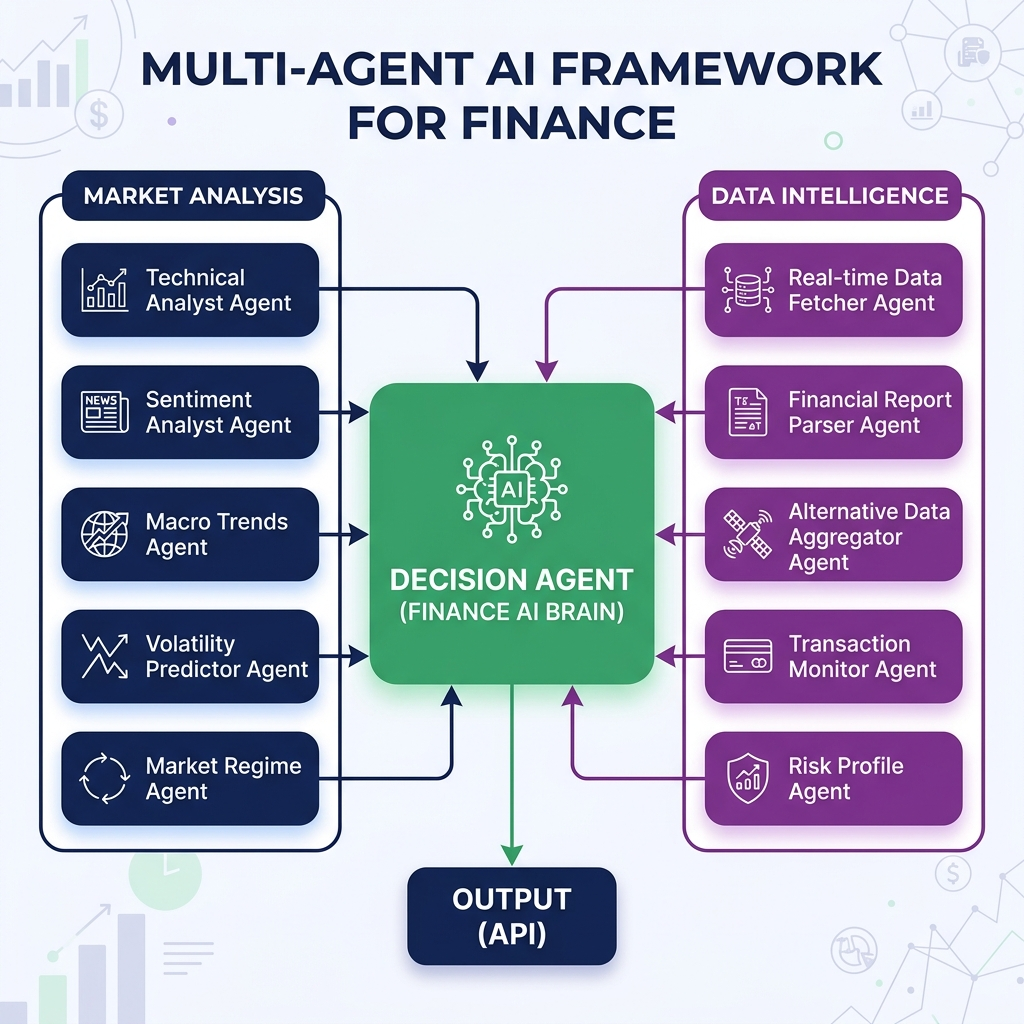
\includegraphics[width=0.85\textwidth]{multi_agent_system.png}
  \caption{13-Agent Consensus System -- Each agent contributes a specialized score to the Decision Agent}
\end{figure}

\begin{figure}[H]
\centering
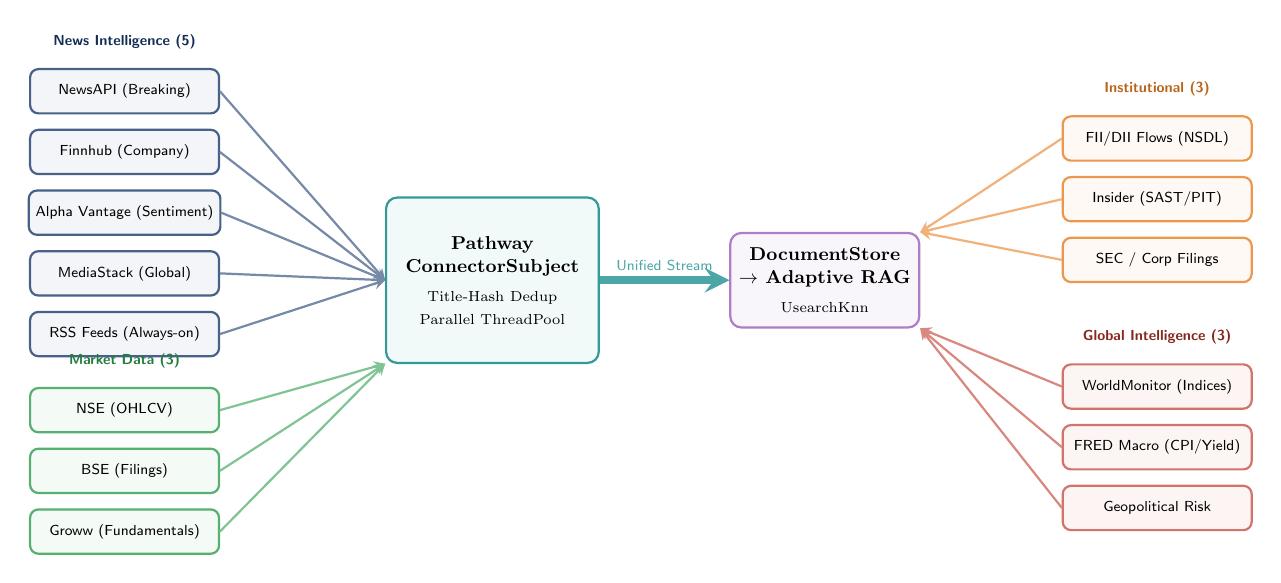
\begin{tikzpicture}[scale=0.75, every node/.style={transform shape},
  node distance=0.4cm,
  srcnavy/.style={draw=navy!80, fill=navy!5, rounded corners=3pt, thick,
              align=center, minimum width=3.2cm, minimum height=0.75cm,
              font=\scriptsize\sffamily},
  srcgreen/.style={draw=green!80, fill=green!5, rounded corners=3pt, thick,
              align=center, minimum width=3.2cm, minimum height=0.75cm,
              font=\scriptsize\sffamily},
  srcorange/.style={draw=orange!80, fill=orange!5, rounded corners=3pt, thick,
              align=center, minimum width=3.2cm, minimum height=0.75cm,
              font=\scriptsize\sffamily},
  srcred/.style={draw=red!70, fill=red!5, rounded corners=3pt, thick,
              align=center, minimum width=3.2cm, minimum height=0.75cm,
              font=\scriptsize\sffamily},
  aggbox/.style={draw=teal!80, fill=teal!5, rounded corners=4pt, thick,
                 align=center, minimum width=3.6cm, minimum height=2.8cm,
                 font=\small\bfseries},
  outbox/.style={draw=purple!70, fill=purple!5, rounded corners=4pt, thick,
                 align=center, minimum width=3.2cm, minimum height=1.6cm,
                 font=\small\bfseries},
  bigarr/.style={->, >=stealth, line width=1mm, teal!70}
]

  % ── Central Aggregator ──
  \node[aggbox] (agg) {Pathway\\ConnectorSubject\\[3pt]
        \normalfont\scriptsize Title-Hash Dedup\\
        \normalfont\scriptsize Parallel ThreadPool};

  % ── Output ──
  \node[outbox, right=2.2cm of agg] (out) {DocumentStore\\$\to$ Adaptive RAG\\[3pt]
        \normalfont\scriptsize UsearchKnn};
  \draw[bigarr] (agg.east) -- (out.west)
    node[midway, above, font=\scriptsize\sffamily\color{teal!70}] {Unified Stream};

  % ── News Intelligence (top-left) ──
  \node[srcnavy, left=2.8cm of agg.west, yshift=3.2cm] (newsapi) {NewsAPI (Breaking)};
  \node[srcnavy, below=0.25cm of newsapi]              (finnhub) {Finnhub (Company)};
  \node[srcnavy, below=0.25cm of finnhub]              (alphav)  {Alpha Vantage (Sentiment)};
  \node[srcnavy, below=0.25cm of alphav]               (media)   {MediaStack (Global)};
  \node[srcnavy, below=0.25cm of media]                (rss)     {RSS Feeds (Always-on)};
  \node[font=\scriptsize\sffamily\bfseries\color{navy!80!black}, above=0.2cm of newsapi] {News Intelligence (5)};

  % ── Market Data (bottom-left) ──
  \node[srcgreen, left=2.8cm of agg.west, yshift=-2.2cm] (nse)   {NSE (OHLCV)};
  \node[srcgreen, below=0.25cm of nse]                  (bse)   {BSE (Filings)};
  \node[srcgreen, below=0.25cm of bse]                  (groww) {Groww (Fundamentals)};
  \node[font=\scriptsize\sffamily\bfseries\color{green!80!black}, above=0.2cm of nse] {Market Data (3)};

  % ── Institutional (top-right) ──
  \node[srcorange, right=2.4cm of out.east, yshift=2.4cm] (fii)     {FII/DII Flows (NSDL)};
  \node[srcorange, below=0.25cm of fii]                   (insider) {Insider (SAST/PIT)};
  \node[srcorange, below=0.25cm of insider]               (sec)     {SEC / Corp Filings};
  \node[font=\scriptsize\sffamily\bfseries\color{orange!80!black}, above=0.2cm of fii] {Institutional (3)};

  % ── Global Intelligence (bottom-right) ──
  \node[srcred, right=2.4cm of out.east, yshift=-1.8cm] (world) {WorldMonitor (Indices)};
  \node[srcred, below=0.25cm of world]                   (macro) {FRED Macro (CPI/Yield)};
  \node[srcred, below=0.25cm of macro]                   (geo)   {Geopolitical Risk};
  \node[font=\scriptsize\sffamily\bfseries\color{red!70!black}, above=0.2cm of world] {Global Intelligence (3)};

  % ── Arrows ──
  \foreach \n in {newsapi,finnhub,alphav,media,rss}
    \draw[->, >=stealth, thick, navy!60] (\n.east) -- (agg.west);
  \foreach \n in {nse,bse,groww}
    \draw[->, >=stealth, thick, green!60] (\n.east) -- (agg.south west);
  \foreach \n in {fii,insider,sec}
    \draw[->, >=stealth, thick, orange!60] (\n.west) -- (out.north east);
  \foreach \n in {world,macro,geo}
    \draw[->, >=stealth, thick, red!60] (\n.west) -- (out.south east);

\end{tikzpicture}%
\caption{AlphaStream ``Herd of Knowledge'' -- 14 Connectors across 4 categories}
\label{fig:herd_knowledge}
\end{figure}

\begin{figure}[H]
\centering
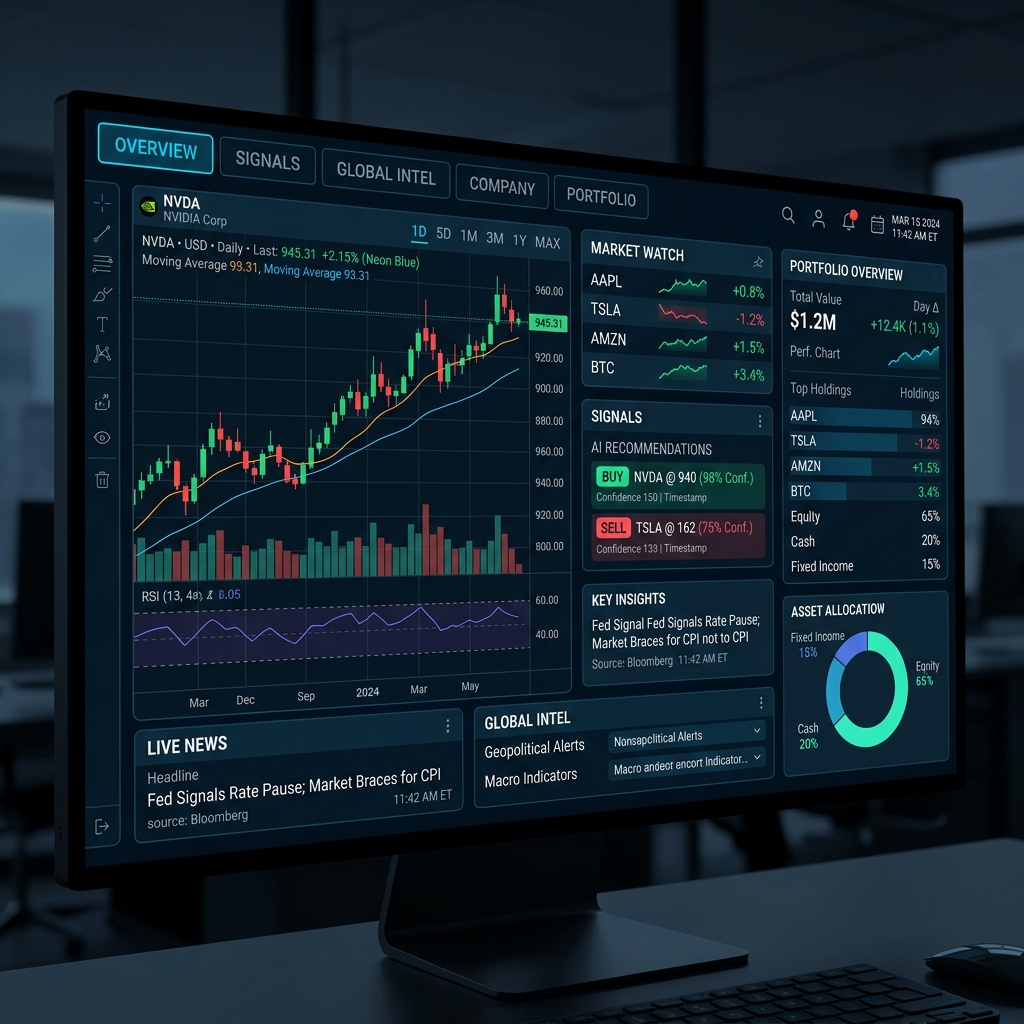
\includegraphics[width=0.95\textwidth]{terminal_ui_mockup.png}
\caption{AlphaStream User Interface -- 5-Tab Bloomberg-Style Terminal}
\label{fig:terminal_impact}
\end{figure}

\begin{figure}[H]
\centering
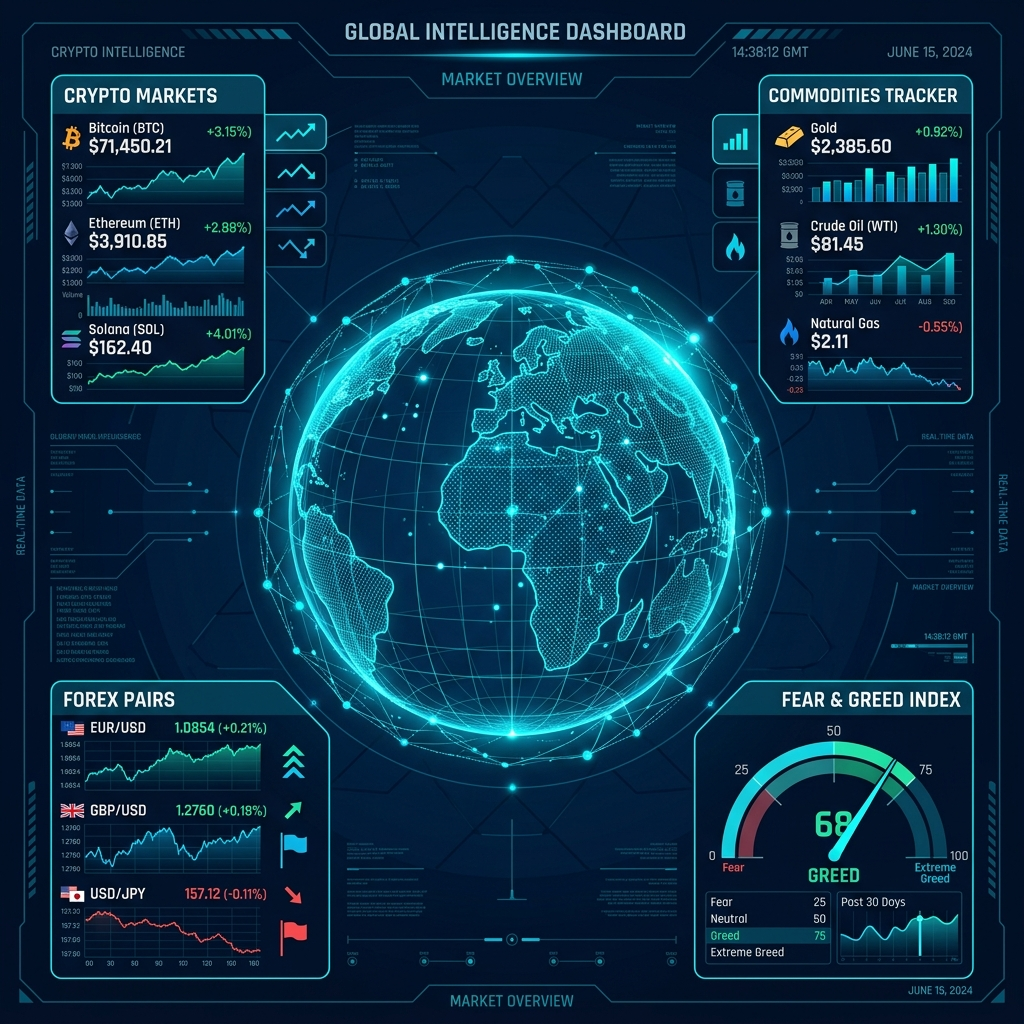
\includegraphics[width=0.85\textwidth]{worldmonitor_dashboard.png}
\caption{WorldMonitor Global Intelligence Dashboard -- Crypto, FX, Commodities, Fear \& Greed}
\label{fig:worldmonitor_impact}
\end{figure}

% ============================================================
\section{Agent Roles}

All 13 agents are stateless Python classes, each specializing in one analytical dimension.
They are invoked in parallel via \texttt{asyncio.gather} and return structured dictionaries.

\begin{center}
\scriptsize
\begin{tabular}{L{2.0cm} L{3.8cm} L{3.2cm} L{3.2cm}}
  \toprule
  \textbf{Agent} & \textbf{Role} & \textbf{Inputs} & \textbf{Outputs} \\
  \midrule
  \textbf{Sentiment} & Scores news sentiment & Retrieved article chunks & sentiment\_score ($-1$ to $+1$),\newline label, key\_factors \\[4pt]
  \textbf{Technical} & Computes RSI, MACD, SMA & yfinance OHLCV & technical\_score, key\_signals \\[4pt]
  \textbf{Risk} & Volatility \& position sizing & Price history & risk\_score, stop\_loss \\[4pt]
  \textbf{Pattern} & Detects 7 chart patterns & 6-month OHLCV & patterns with confidence \\[4pt]
  \textbf{Backtest} & Validates signals historically & Pattern + 5yr OHLCV & win\_rate, avg\_return, sharpe \\[4pt]
  \textbf{Flow} & FII/DII institutional streaks & NSDL flow data & flow\_signal, streak\_days \\[4pt]
  \textbf{Filing} & Classifies BSE/NSE filings & Announcement text & materiality, sentiment \\[4pt]
  \textbf{Insider} & Parses NSE SAST/PIT data & NSE insider trades & insider\_score, transactions \\[4pt]
  \textbf{Anomaly} & Online anomaly detection & Price, volume, sentiment & anomaly\_flags, drift\_alerts \\[4pt]
  \textbf{Search} & Web context enrichment & NLQ query & title, url, snippet \\[4pt]
  \textbf{Chart} & Generates annotated charts & yfinance OHLCV & PNG chart path \\[4pt]
  \textbf{Report} & Generates PDF reports & All agent outputs & PDF report path \\[4pt]
  \textbf{Decision} & Final BUY/HOLD/SELL & All agent outputs & recommendation, confidence,\newline reasoning, Alpha Score \\
  \bottomrule
\end{tabular}
\end{center}

% ============================================================
\section{Agent Communication}

Agents are \textbf{stateless} -- no message broker is used. The orchestrator
(\texttt{generate\_recommendation\_logic()}) calls each agent in order and passes
results forward via Python dictionaries.

\subsection{Recommendation Path}

\begin{center}
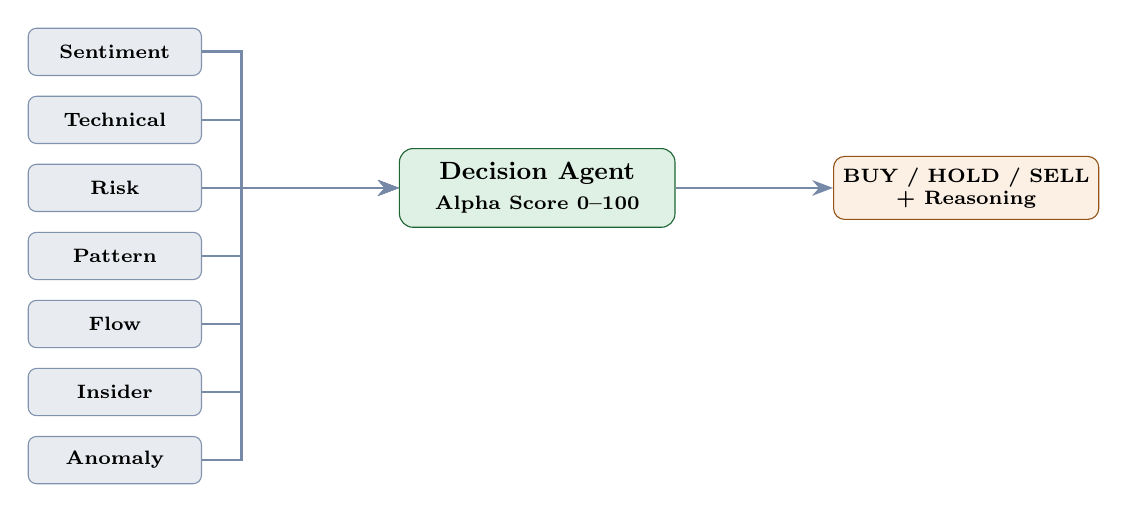
\begin{tikzpicture}[node distance=0.3cm and 0.5cm,
  agentsmall/.style={draw=navy!55, fill=navy!10,
    rounded corners=3pt, minimum width=2.2cm, minimum height=0.6cm,
    align=center, font=\scriptsize\bfseries},
  decbox/.style={draw=green!65!black, fill=green!15,
    rounded corners=5pt, minimum width=3.5cm, minimum height=1cm,
    align=center, font=\small\bfseries},
  outbox/.style={draw=orange!65!black, fill=orange!12,
    rounded corners=4pt, minimum width=3cm, minimum height=0.8cm,
    align=center, font=\scriptsize\bfseries},
  arr/.style={->, >=Stealth, line width=1pt, color=navy!60}]

  \node[agentsmall] (s) {Sentiment};
  \node[agentsmall, below=0.25cm of s] (t) {Technical};
  \node[agentsmall, below=0.25cm of t] (r) {Risk};
  \node[agentsmall, below=0.25cm of r] (p) {Pattern};
  \node[agentsmall, below=0.25cm of p] (f) {Flow};
  \node[agentsmall, below=0.25cm of f] (i) {Insider};
  \node[agentsmall, below=0.25cm of i] (a) {Anomaly};

  \node[decbox, right=2.5cm of r] (dec) {Decision Agent\\{\scriptsize Alpha Score 0--100}};
  \node[outbox, right=2cm of dec] (out) {BUY / HOLD / SELL\\+ Reasoning};

  \draw[arr] (s.east) -- ++(0.5,0) |- (dec.west);
  \draw[arr] (t.east) -- ++(0.5,0) |- (dec.west);
  \draw[arr] (r.east) -- (dec.west);
  \draw[arr] (p.east) -- ++(0.5,0) |- (dec.west);
  \draw[arr] (f.east) -- ++(0.5,0) |- (dec.west);
  \draw[arr] (i.east) -- ++(0.5,0) |- (dec.west);
  \draw[arr] (a.east) -- ++(0.5,0) |- (dec.west);

  \draw[arr] (dec.east) -- (out.west);

\end{tikzpicture}
\end{center}

\subsection{NLQ Path (Separate)}

The NLQ path is independent: \texttt{NLQ Router $\to$ Text2SQL / Pre-defined SQL $\to$
DuckDB $\to$ Narrate $\to$ SSE stream}. The \texttt{SearchAgent} is called as optional
enrichment when the local DuckDB result set has fewer than 5 rows.

\subsection{Real-Time Update Path}

Pathway runs in a background daemon thread and fires \texttt{on\_new\_article} callbacks
that trigger recommendation refreshes via \texttt{asyncio.run\_coroutine\_threadsafe}.
Updated recommendations are broadcast to all connected clients over WebSocket
(\texttt{/ws/stream/\{ticker\}}).

% ============================================================
\section{Tool Integrations}

\begin{center}
\small
\begin{tabular}{L{4.5cm} L{9cm}}
  \toprule
  \textbf{Tool / Service} & \textbf{Purpose in AlphaStream} \\
  \midrule
  Pathway \texttt{ConnectorSubject} & Multi-source streaming news ingestion (5 APIs in parallel) \\
  Pathway \texttt{pw.io.subscribe} & Article-arrival callbacks to RAG pipeline \\
  Adaptive RAG Server (port 8001) & Pathway-powered vector search with incremental indexing \\
  DuckDB & Structured market data store (prices, signals, filings, FII/DII) \\
  ChromaDB & Dense vector index for semantic article retrieval \\
  FastMCP servers (4 servers) & Market data, signals, portfolio, search tools for NLQ \\
  yfinance & OHLCV price data (\texttt{.NS} suffix for NSE tickers) \\
  NSE / BSE APIs & Insider trades (SAST/PIT), corporate filings, FII/DII flows \\
  Groww API & Live fundamentals (PE, PB, ROE) via JWT + TOTP auth \\
  River ML & Incremental online ML (HalfSpaceTrees) for AnomalyAgent \\
  FRED API & US macro indicators (CPI, yield curve, unemployment) \\
  CNN Fear \& Greed & Market sentiment gauge (0--100 index) \\
  WorldMonitor / yfinance & Global indices, crypto, commodities, FX rates \\
  LangChain + LangGraph & Agent orchestration + NLQ 8-node pipeline \\
  Gemini 2.0 Flash (Vertex AI) & LLM reasoning for all agents \\
  \bottomrule
\end{tabular}
\end{center}

% ============================================================
\section{Error-Handling Logic}

\begin{center}
\small
\begin{tabular}{L{4cm} L{9.5cm}}
  \toprule
  \textbf{Failure Scenario} & \textbf{Handling Strategy} \\
  \midrule
  Pathway unavailable & Skipped at startup; news ingestion falls back to polling connector \\[3pt]
  Adaptive RAG server not ready & \texttt{UnifiedRAGService} falls back to manual ChromaDB RAG \\[3pt]
  LLM timeout in any agent & Agent returns safe default (HOLD / score 0.0); exception logged, not re-raised \\[3pt]
  Text2SQL generates bad SQL & Correction loop: classify error $\to$ LLM fix $\to$ retry (max 2 attempts) \\[3pt]
  DuckDB query timeout & Hard 30s limit, 5000-row cap; error returned to user as plain text \\[3pt]
  NSE API blocked & yfinance \texttt{.NS} suffix as fallback for price data \\[3pt]
  MCP server crash & Agent degrades gracefully -- direct DuckDB queries used instead \\[3pt]
  WebSocket disconnect & \texttt{ConnectionManager.disconnect()} removes client; server continues \\[3pt]
  Missing GCP credentials & Pydantic \texttt{model\_validator} warns at startup \\[3pt]
  Graceful shutdown & \texttt{SIGINT/SIGTERM} handler kills Pathway subprocess and waits \\
  \bottomrule
\end{tabular}
\end{center}

\newpage

% ============================================================
%  PART 2: IMPACT MODEL
% ============================================================

\section{Impact Model}

\begin{keymetricbox}
\centering
\begin{tabular}{cccc}
  {\LARGE\bfseries\color{navy}\Rs{}2.19L} &
  {\LARGE\bfseries\color{green}\Rs{}54K} &
  {\LARGE\bfseries\color{orange}\Rs{}59.9 Cr} &
  {\LARGE\bfseries\color{purple}15\%} \\[3pt]
  {\scriptsize\color{steel}Time Saved/User/Year} &
  {\scriptsize\color{steel}Alpha/User/Year} &
  {\scriptsize\color{steel}Year 1 Revenue} &
  {\scriptsize\color{steel}Risk Reduction}
\end{tabular}
\end{keymetricbox}

\subsection{Problem Scale}

\begin{itemize}[leftmargin=1.6em, itemsep=2pt]
  \item \textbf{14 Cr+} demat accounts in India (CDSL + NSDL)
  \item \textbf{$\sim$3 Cr} active traders who research daily
  \item Average retail investor spends \textbf{2+ hours/day} on research
  \item \textbf{80\%} rely on WhatsApp tips and unverified sources
  \item Average missed opportunity cost: \textbf{\Rs{}3,000--10,000/quarter}
\end{itemize}

\subsection{Market Opportunity (TAM / SAM / SOM)}

\begin{center}
\small
\begin{tabular}{L{1.5cm} L{5cm} C{2.5cm} L{4.5cm}}
  \toprule
  \textbf{Level} & \textbf{Segment} & \textbf{Size} & \textbf{Rationale} \\
  \midrule
  \textbf{TAM} & Total Indian equity participants & 14 Cr & CDSL + NSDL demat accounts (2024) \\
  \textbf{SAM} & Active traders researching daily & $\sim$3 Cr & $\approx$20\% trade monthly \\
  \textbf{SOM} & 5-year premium capture & 1.5 L & 0.5\% of SAM (conservative) \\
  \bottomrule
\end{tabular}
\end{center}

\noindent
\small\textit{Key: SOM uses 0.5\% of SAM, not TAM -- anchored to paying users, not total accounts.}

\subsection{Time Saved}

\begin{greenbox}[title={Time Value Recovered Per User}]
\textbf{1.75 hours/day} $\times$ \Rs{}500/hr $\times$ 250 trading days
$= \mathbf{\Rs{}2.19\ Lakh/user/year}$ in recovered productivity.
\end{greenbox}

\begin{center}
\small
\begin{tabular}{L{4.5cm} L{3.5cm} L{3.5cm}}
  \toprule
  \textbf{Task} & \textbf{Without AlphaStream} & \textbf{With AlphaStream} \\
  \midrule
  Daily market research      & 2+ hours         & 15 minutes \\
  Corporate filing analysis  & 30 min/filing    & Instant LLM classification \\
  Insider trade monitoring   & Manual NSE checks & Automated alerts \\
  FII/DII tracking           & Visit NSDL daily  & Real-time flow analysis \\
  Signal identification      & Manual chart reading & Automated pattern scan \\
  \bottomrule
\end{tabular}
\end{center}

\subsection{Alpha Generated (Revenue Recovered)}

\begin{center}
\small
\begin{tabular}{L{3.5cm} L{3.5cm} C{2cm} C{3cm}}
  \toprule
  \textbf{Signal Type} & \textbf{Detection} & \textbf{Win Rate} & \textbf{Avg 30d Return} \\
  \midrule
  RSI Divergence      & Automated scan   & 60--78\% & +3.26\% \\
  MACD Crossover      & Real-time detect.& 45--57\% & +0.71\% \\
  Insider Cluster Buy & 3+ insiders/30d  & High (historical) & Varies \\
  FII Buying Streak   & 5+ consecutive sessions & $\sim$72\% & +3--5\% \\
  \bottomrule
\end{tabular}
\end{center}

\begin{orangebox}[title={Conservative Alpha Estimate}]
2--3 actionable signals/month $\times$ 60\% accuracy $\times$ \Rs{}3,000 average gain
$= \mathbf{\Rs{}54,000/user/year}$ in additional alpha (revenue recovered from missed opportunities).
\end{orangebox}

\subsection{Risk Reduction (Cost Reduced)}

\begin{itemize}[leftmargin=1.6em, itemsep=2pt]
  \item \textbf{Early warning} on adverse signals prevents panic selling
  \item \textbf{Portfolio-aware alerts}: ``Your IT holdings at risk from FII selling streak''
  \item \textbf{Backtested confidence}: ``This pattern has worked 78\% of the time on this stock''
  \item Estimated \textbf{15\% reduction} in behavioral losses (fear-driven selling, FOMO buying)
\end{itemize}

\subsection{ET Markets Revenue Projection}

\begin{center}
\small
\begin{tabular}{L{5.5cm} C{2.3cm} C{2.3cm} C{2.3cm}}
  \toprule
  & \textbf{Year 1} & \textbf{Year 3} & \textbf{Year 5} \\
  \midrule
  Premium users (\Rs{}999/month) & 50,000 & 2,00,000 & 5,00,000 \\
  \textbf{Annual Revenue}        & \textbf{\Rs{}59.9 Cr} & \textbf{\Rs{}239.8 Cr} & \textbf{\Rs{}599.4 Cr} \\
  \midrule
  Increased engagement           & +40\% time on platform & -- & -- \\
  Reduced churn                  & 2x retention & -- & -- \\
  \bottomrule
\end{tabular}
\end{center}

\subsection{Cost Reduction for ET Markets}

\begin{center}
\small
\begin{tabular}{L{3.5cm} L{3.5cm} L{3.5cm} L{2.5cm}}
  \toprule
  \textbf{Cost Category} & \textbf{Current Approach} & \textbf{With AlphaStream} & \textbf{Saving} \\
  \midrule
  Signal content & Manual analyst & LLM-generated, & \Rs{}5--10 Cr/yr \\
  (est. \Rs{}20 Cr/yr) & teams + editorial & human-reviewed & (30\% reduction) \\
  \bottomrule
\end{tabular}
\end{center}

\noindent
\small\textit{Automated pipelines handle repeatable content (FII flows, insider alerts, technical scans).
Humans focus on narrative and investigative work -- higher value, lower volume.}

\subsection{Competitive Moat}

\begin{enumerate}[leftmargin=1.8em, itemsep=3pt]
  \item \textbf{India-specific regulatory data} -- NSE SAST/PIT and NSDL FII/DII feeds
        not available through generic global APIs.
  \item \textbf{Backtested signals, not LLM speculation} -- every signal carries a win rate
        grounded in NSE/BSE historical data; LLM-only tools cannot replicate this.
  \item \textbf{Streaming architecture} -- Pathway incremental indexing achieves $<$2s
        latency vs.\ static dashboards that recompute on every page load.
  \item \textbf{Portfolio-aware alerts} -- signals contextualised to each user's
        actual holdings, not generic screener results.
  \item \textbf{Compound improvement} -- each user interaction improves signal ranking;
        system accuracy scales with user base.
\end{enumerate}

\subsection{Assumptions (Stated Explicitly)}

\begin{enumerate}[leftmargin=1.8em, itemsep=1pt]
  \item Win rates based on backtesting against Nifty 50 stocks with 3--5 year data
  \item Average return estimates use median, not mean (to reduce outlier effect)
  \item Time savings assumes basic digital literacy and daily market participation
  \item Premium conversion rate of 0.3\% is conservative (industry average is 0.5--1\%)
  \item Back-of-envelope calculations -- detailed validation would require A/B testing
  \item SOM (1.5L users) = 0.5\% of SAM (3 Cr active traders) -- conservative for a 5-year horizon
  \item Revenue projections assume no price increase over 5 years (understates upside)
  \item Cost reduction estimate assumes research content budget of $\sim$\Rs{}20 Cr/year at ET Markets' scale
  \item Year 3 and Year 5 user projections assume compounding growth of $\sim$100\% and $\sim$150\% respectively from Year 1 base
\end{enumerate}

\vfill
\begin{center}
  {\color{cyan}\rule{0.6\linewidth}{0.8pt}}\\[4pt]
  {\small\color{mgray}AlphaStream India \textbullet{} ET AI Hackathon 2026 \textbullet{}
   Problem Statement 6: AI for the Indian Investor}\\[2pt]
  {\small\color{navy}\url{https://github.com/wildcraft958/AlphaStream_India}}
\end{center}

\end{document}
